% CONCISE VERSION (if space is limited)

\begin{figure}[htbp]
    \centering
    \begin{subfigure}[b]{0.48\textwidth}
        \includegraphics[width=\textwidth]{figures/Fig_Variance_Explained_30.png}
        \caption{30-dimensional latent space}
    \end{subfigure}
    \hfill
    \begin{subfigure}[b]{0.48\textwidth}
        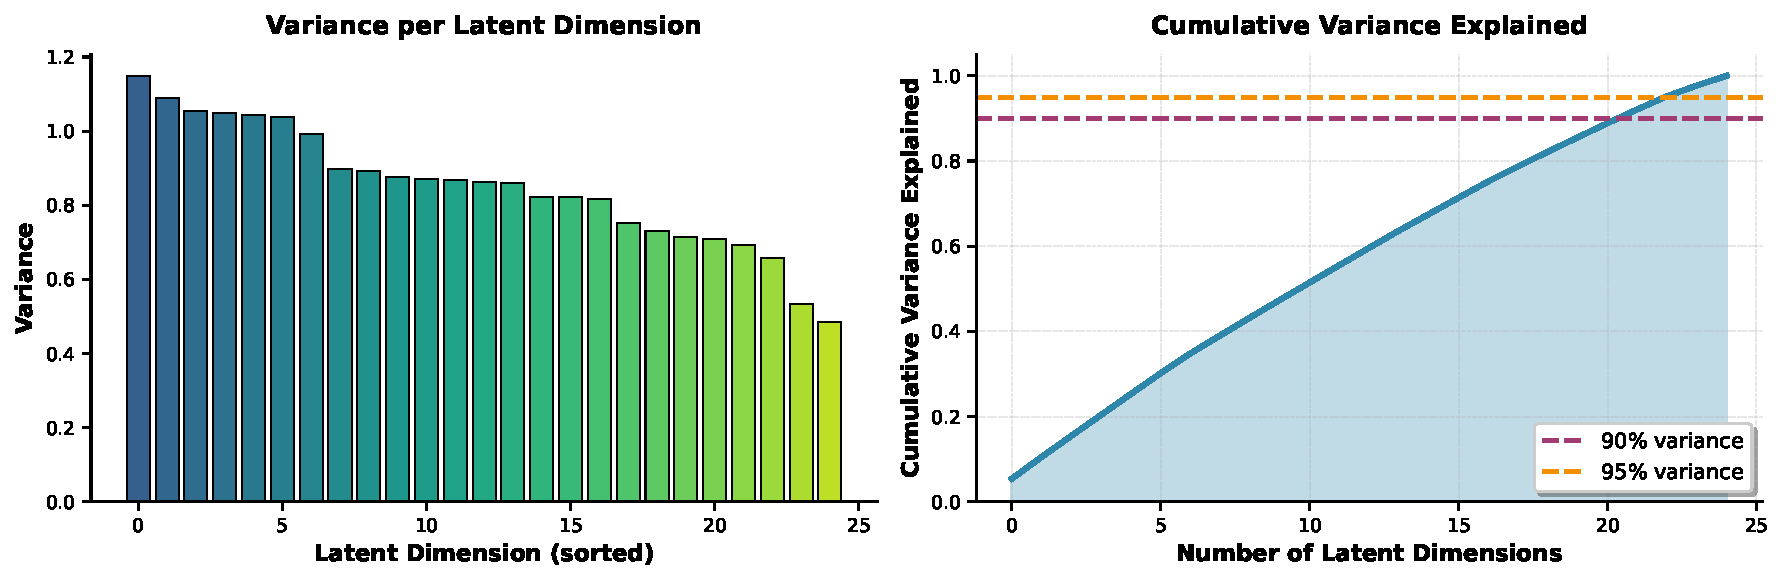
\includegraphics[width=\textwidth]{figures/Fig_Variance_Explained.png}
        \caption{50-dimensional latent space}
    \end{subfigure}
    \caption{\textbf{Latent space variance distribution.}
    \textbf{Left:} Per-dimension variance (sorted) shows hierarchical information encoding with few dimensions capturing most variability.
    \textbf{Right:} Cumulative variance indicates $\sim$20--25 dimensions capture 90\% of variance.
    The 30-dimensional configuration \textbf{(a)} provides efficient encoding comparable to the 50-dimensional space \textbf{(b)}, justifying the model's architecture choice.}
    \label{fig:variance_explained}
\end{figure}
